\chapter{Statica}

Obiettivo della statica è la \textbf{determinazione delle relazioni fra le forze e le coppie applicate sulla punta operativa e le forze e le coppie applicate ai giunti}, quando il manipolatore si trova in una \textbf{configurazione di equilibrio} (i.e. quando tutto è fermo).

Chiamiamo \textbf{forze generalizzate} il vettore composto di forze e coppie (torques) assieme (tecnicamente questo non sarebbe un vettore perchè gli elementi hanno unità di misure diverse: forze in $N$, coppie in $Nm$).

Indicheremo con
$$
\bm{F}
\triangleq
\begin{bmatrix*}
\bm{f}(t) \\
\bm{N}(t)
\end{bmatrix*}
\qquad
\bm{f},\bm{N} \in \R^3
$$
($f$ forze, $N$ momenti) il vettore delle \textbf{forze generalizzate cartesiane} applicate sulla punta operativa (task space generalized forces (\textbf{TSGF})), mentre con
$$
\bm{\tau}(t)
\triangleq
\begin{bmatrix*}
	\tau_1 \\
	\vdots \\
	\tau_n
\end{bmatrix*}
$$
il vettore delle \textbf{forze generalizzate ai giunti} (joint generalized forces (\textbf{JGF})); visto che i giunti maggiormente impiegati sono di tipo rotoidale, $\bm{\tau}(t)$ è spesso indicato come vettore delle \textbf{coppie generalizzate}.

\begin{itemize}
	\item Per \textbf{giunti prismatici}: 
	$$
	\tau_i = \bm{k}^T_{i-1} \bm{f}_{i-1,i}
	$$
	\item Per \textbf{giunti rotoidali}: 
	$$
	\tau_i = \bm{k}^T_{i-1} \bm{N}_{i-1,i}
	$$
\end{itemize}


Le TSGF sono generate dalle interazioni della punta con l'ambiente (e.g. quando il TCP preme contro una superficie), mentre le JGF sono generate dalla potenza sviluppata dai motori.

\begin{figure}[H]
	\centering
	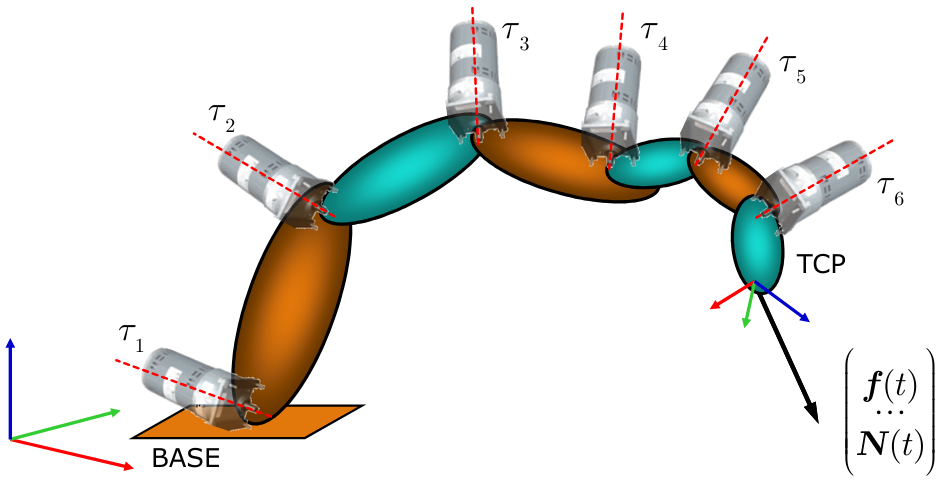
\includegraphics[width=0.7\linewidth]{images/statics_1}
	\caption{Statics}
	\label{fig:statics1}
\end{figure}

\section{Relazione fra $F$ e $\tau$}
Per trovare questa relazione possiamo usare il \textbf{principio dei lavori virtuali}:
\begin{itemize}
	\item Il \textbf{lavoro} è una grandezza reale data dal prodotto di una forza per uno spostamento lineare oppure dal prodotto di un momento per uno spostamento angolare
	\item Il \textbf{lavoro virtuale} è quello associato agli spostamenti virtuali, dati da tutti i possibili spostamenti geometrici compatibili con gli eventuali vincoli sul sistema
\end{itemize}
Il lavoro virtuale nasce dall'applicazione del \textbf{principio di minima azione} allo studio delle forze e del movimento di un sistema meccanico. Il lavoro di una forza che agisce su una particella mentre si muove lungo uno spostamento è diverso a seconda degli spostamenti. Tra tutti i possibili spostamenti che una particella può seguire, detti \textbf{spostamenti virtuali}, quello ne minimizzerà l'azione. Questo spostamento è quindi lo spostamento seguito dalla particella secondo il principio di minima azione. Il lavoro di una forza su una particella lungo uno spostamento virtuale è noto come lavoro virtuale.

Sia
$$
\delta W_{TCP} = \bm{F}^T\delta\bm{p}
$$
il lavoro virtuale associato alle forze generalizzate cartesiane, dove $\delta\bm{p}$ è lo spostamento virtuale cartesiano (formato dagli spostamenti virtuali lineare ed angolare). 
\begin{figure}[H]
	\centering
	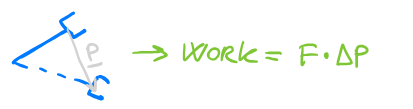
\includegraphics[width=0.3\linewidth]{images/statics_2}
	\label{fig:statics2}
\end{figure}

Sia anche
$$
\delta W_{g} = \bm{\tau}^T\delta\bm{q}
$$
il lavoro virtuale associato alle forze generalizzate ai giunti, ove $\delta\bm{q}$ è lo spostamento virtuale ai giunti.
Secondo il \textbf{principio dei lavori virtuali}, il manipolatore è in condizioni di equilibrio statico se e solo se i lavori virtuali delle forze generalizzate cartesiane e ai giunti sono uguali, qualunque sia la configurazione del robot:
$$
\delta W_g = \delta W_{TCP}
\iff
\bm{\tau}^T\delta \bm{q} = \bm{F}^T\delta\bm{p} \ \forall \bm{q}(t)
$$
Ora, visto che il nostro manipolatore è rappresentato da un sistema tempo-invariante (la configurazione dipenda da $\bm{q}(t)$, ma non esplicitamente dal tempo), possiamo dire che gli spostamenti virtuali coincidono con gli spostamenti elementari:
$$
\delta\bm{p}= d \bm{p}, \ \delta\bm{q} = d\bm{q}
$$

Richiamando $v=J(q)\dot{q}$ e che $v = dp/dt$, abbiamo:
$$
\bm{v} = \bm{J}(\bm{q})\bm{\dot{q}}
\iff
\frac{d\bm{p}}{\cancel{dt}} = \bm{J}(\bm{q}) \frac{d\bm{q}}{\cancel{dt}}
\iff
d\bm{p} = \bm{J}(\bm{q}) d\bm{q}
$$
dal principio dei lavori virtuali però abbiamo che  $\bm{F}^Td\bm{p} = \bm{\tau}^Td \bm{q}$, e quindi:
$$
d\bm{p} = \bm{J}(\bm{q}) d\bm{q}
\iff
\bm{\tau}d\bm{q} = \bm{F}^T\bm{J}(\bm{q})d\bm{q}
\iff
\bm{\tau}^T = \bm{F}^T\bm{J}
\iff
\bm{\tau} = \bm{J}^T\bm{F}
$$
Quindi, le forze ai giunti necessarie per bilanciare le forze sul TCP sono date da:
\begin{equation}\label{eq:static_equivalence}
\boxed{
\bm{\tau} = -\bm{J}^T(\bm{q})\bm{F}
}
\end{equation}
che è proprio la relazione statica cercata.




\section{Dualità cineto-statica}
In algebra lineare, 
$$
y = A^Tx \quad \text{è il problema duale di} \quad y = Ax
$$
quindi, dalla seguente osservazione:
\begin{figure}[H]
	\centering
	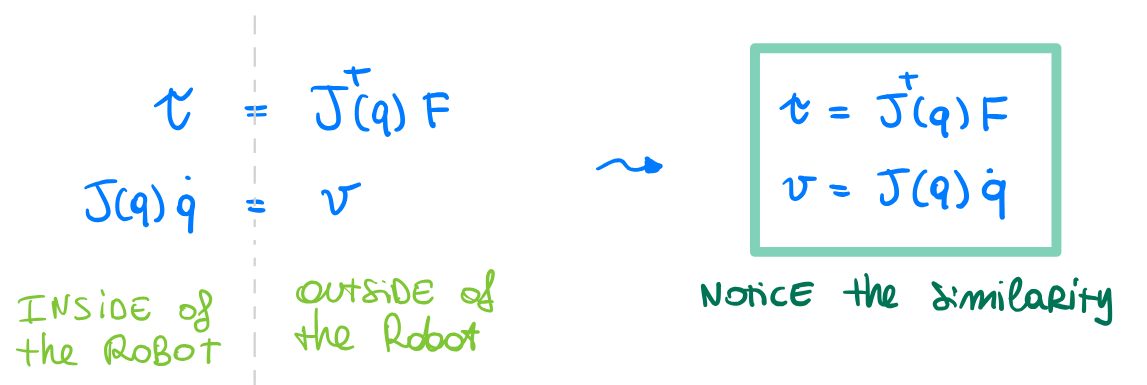
\includegraphics[width=0.7\linewidth]{images/statics_3}
	\label{fig:statics3}
\end{figure}
notiamo che possiamo vedere la relazione statica come il duale del problema della cinematica diretta delle velocità.

Prendiamo 
$$
\bm{F}^* \in \mathcal{N}(\bm{J}^T) \qquad s.t. \qquad \bm{J}^T\bm{F}^* = 0
$$
dalla relazione statica possiamo dire che $\bm{F}^*$ è un vettore di forze (applicate al TCP) che \underline{non} richiede alcuna compensazione dai motori: un esempio può essere visto in fig. \ref{fig:statics4}, dove abbiamo il braccio di un manipolatore a "penzoloni"; in questo caso abbiamo la forza di gravità che "tira" in giù, ma non sono necessarie alcune compensazioni da parte dei motori.
\begin{figure}[H]
	\centering
	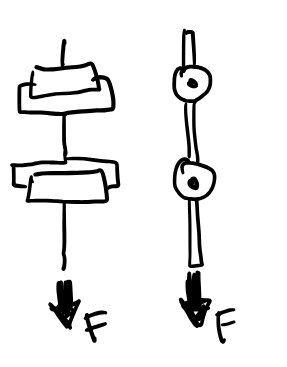
\includegraphics[width=0.2\linewidth]{images/statics_4}
	\caption{Esempio}
	\label{fig:statics4}
\end{figure}


Detto questo possiamo ora parlare più in dettaglio della relazione matematica che esiste fra $\bm{\tau}$ e $\bm{v}$. La dualità può essere caratterizzata dal range ed il kernel di $\bm{J}$ e $\bm{J}^T$:
\begin{itemize}
	\item $\mathcal{R}(\bm{J})$: velocità del TCP che possono essere raggiunte per una data posa
	\item $\mathcal{N}(\bm{J})$: velocità dei giunti che \underline{non} producono alcuna velocità nel TCP (per la data posa)
	\item $\mathcal{R}(\bm{J}^T)$: JFG ($\tau$) che riscono a bilanciare le forze generalizzate applicate al TCP ($F$), per la posa corrente
	\item $\mathcal{N}(\bm{J}^T)$: forze generalizzate applicate al TCP ($F$) che \underline{non} richiedono compensazione di JFG/coppie ($\tau$) (per la data posa)
\end{itemize}
Da algebra lineare, ricordiamo che:
$$
\mathcal{N}(\bm{J}) \equiv \mathcal{R}^\perp(\bm{J}^T)
\qquad
\mathcal{R}(\bm{J}) \equiv \mathcal{N}^\perp(\bm{J}^T)
$$
Da qui segue che, \textbf{quando il manipolatore è in configurazione singolare}:
\begin{itemize}
	\item Esistono velocità non nulle ai giunti $\dot{\bm{q}} \in \mathcal{N}(\bm{J})$ che producono velocità nulle della punta e \textbf{coppie generalizzate ai giunti} $\bm{\tau} \in \mathcal{N}(\bm{J}) = \mathcal{R}^\perp(\bm{J}^T)$ che non possono essere compensate da alcuna forza generalizzata sulla punta
	\item \textbf{Esistono forze generalizzate} $\bm{F} \in \mathcal{N}(\bm{J}^T)$ che non richiedono alcuna coppia ai giunti per essere bilanciata e velocità della punta operativa $\bm{v} = \mathcal{N}(\bm{J}^T) = \mathcal{R}^\perp(\bm{J})$ che non possono essere ottenute da velocità ai giunti
\end{itemize}




\section{Ellipsoidi di manipolabilità}

\subsection{Velocità}

Spesso, per sistemi lineari SISO, se ne studia il comportamento tramite la cosiddetta risposta all'impulso, che essenzialmente caratterizza il modo in cui il sistema risponde a un'unità di ingresso. Nel caso MIMO, invece (come per un manipolatore), il concetto analogo è quello di caratterizzare l'output in termini di un input con norma unitaria. Consideriamo quindi l'insieme di tutte le velocità dei giunti del robot $\bm{\dot{q}}$ tali che:
$$
\|\bm{\dot{q}}\|^2
= 
\dot{q}_1^2 + \dots + \dot{q}_n^2 
\ 
\leq 1
\iff
\bm{\dot{q}}^T\bm{\dot{q}} = 1
$$
usando $\bm{\dot{q}} = \bm{J}^\dagger \bm{v}$, si ottiene:
$$
\bm{\dot{q}}^T\bm{\dot{q}}
=
(\bm{J}^\dagger\bm{v})^T (\bm{J}^\dagger \bm{v})
=
\bm{v}^T (\bm{J}\bm{J}^T)^{-1}\bm{v}
$$
possiamo quindi definire il \textbf{velocity manipulability ellipsoid} come quei punti che soddisfano:
$$
E_v = \{\bm{v} \ : \ \bm{v}^T (\bm{J}\bm{J}^T)^{-1}\bm{v} = 1 \}
$$
notare che varia con il variare di $\bm{q}$. Da qui possiamo anche definire un'altro valore utile, chiamato \textbf{manipulability measure}:
$$
w(\bm{q}) = \sqrt{\det(\bm{J}\bm{J}^T)}
=
|\lambda_1\lambda_2 \cdots \lambda_n|
=
|\det(\bm{J})|
$$
che non è altro che il volume dell'ellissoide definito prima ($\lambda_i$ sono gli autovalori di $\bm{J}$).

Un'interessante osservazione può essere fatta per le \textbf{singolarità}: quando il manipolatore approccia una postura singolare abbiamo che $\lambda_i \to 0$ e quindi anche $w(\bm{q}) \to 0$ (non abbiamo manipolabilità!). Per questo motivo $w(\bm{q})$ è spesso usata come misura di "distanza" dalle configurazioni singolari.

\begin{figure}
	\centering
	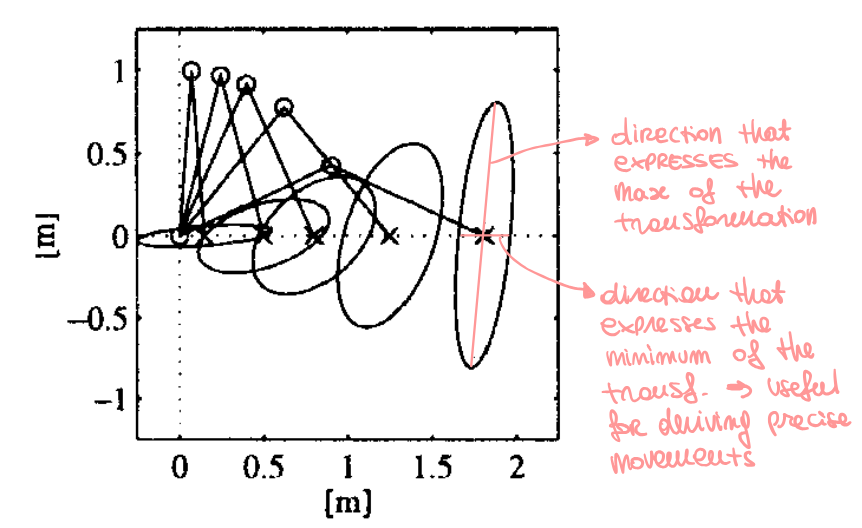
\includegraphics[width=0.6\linewidth]{images/statics_5}
	\caption{Ellissoidi di manipolabilità al variare della postura per un manipolatore con 2 giunti}
	\label{fig:statics5}
\end{figure}





\subsection{Forza}

Dalla dualità cineto-statica possiamo derivare un ellissoide di manipolabilità anche per le forze. Questa volta invece delle velocità dei giunti andiamo ad utilizzare le coppie generalizzate ai giunti:
$$
\bm{\tau}^T\bm{\tau} = 1
$$
allora, il \textbf{force manipulability ellipsoid} è definito come:
$$
E_F = \{\bm{F} \ : \ \bm{F}^T (\bm{J}\bm{J}^T)\bm{F} = 1 \}
$$
dove abbiamo utilizzato $\bm{\tau} = \bm{J}^T\bm{F}$.

\begin{figure}[H]
	\centering
	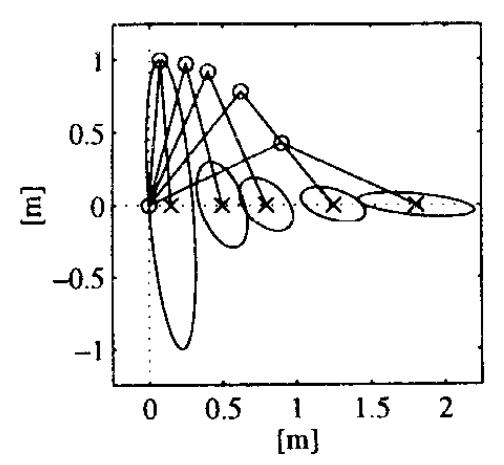
\includegraphics[width=0.3\linewidth]{images/statics_6}
	\caption{Stesso esempio di prima ma per la forza}
	\label{fig:statics6}
\end{figure}

Comparando la definizione di $E_F$ con quella di $E_v$ possiamo notare che in questo caso il contenuto fra le parentesi ($JJ^T$) non è invertito (mentre prima si): da qui consegue l'importante fatto che gli assi principali dell'ellissoide di manipolabilità della forza coincidono con quelli della velocità, ma con valori "inversi".\\
Da questo consegue un risultato anche intuitivo: \textbf{una direzione dove abbiamo una buona manipolabilità in velocità avrà cattiva manipolabilità di forza, e viceversa} $\rightarrow$ \textbf{veloce e debole \textit{oppure} lento e forte} (\textit{pensa al cambio di una bici/auto: in salita vado lento ma faccio tanta forza, in piano faccio meno forza ma vado più veloce}).

\begin{figure}
	\centering
	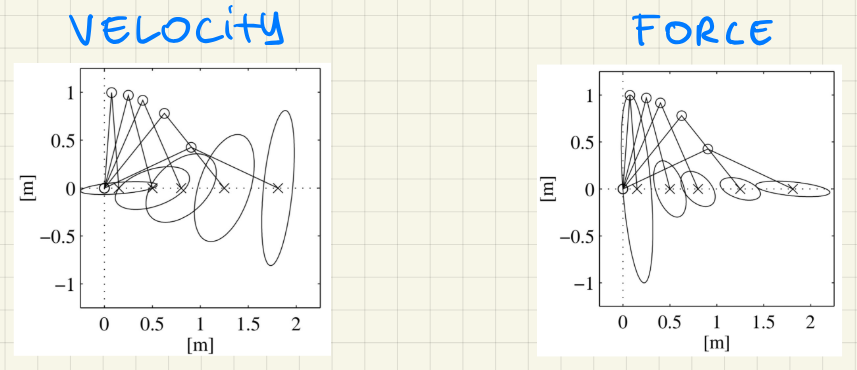
\includegraphics[width=0.6\linewidth]{images/statics_7}
	\caption{Comparazione: notare l'"inversione" fra i due}
	\label{fig:statics7}
\end{figure}


